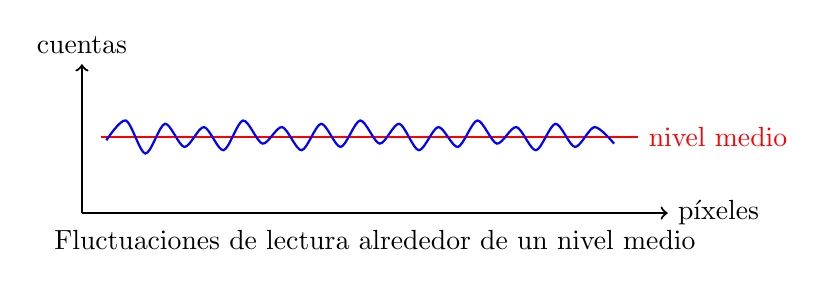
\begin{tikzpicture}[x=0.62cm,y=0.42cm]
  \draw[->,thick] (0,0) -- (12,0) node[right] {píxeles};
  \draw[->,thick] (0,0) -- (0,4.5) node[above] {cuentas};
  \draw[red,thick] (0.4,2.3) -- (11.4,2.3) node[right] {nivel medio};
  \draw[blue,thick,smooth] plot coordinates {
    (0.5,2.2) (0.9,2.8) (1.3,1.8) (1.7,2.7) (2.1,2.0)
    (2.5,2.6) (2.9,1.9) (3.3,2.8) (3.7,2.1) (4.1,2.6)
    (4.5,1.9) (4.9,2.7) (5.3,2.0) (5.7,2.8) (6.1,2.1)
    (6.5,2.7) (6.9,1.9) (7.3,2.6) (7.7,2.0) (8.1,2.8)
    (8.5,2.1) (8.9,2.6) (9.3,1.9) (9.7,2.7) (10.1,2.0)
    (10.5,2.6) (10.9,2.1)
  };
  \node[align=center] at (6,-0.8) {Fluctuaciones de lectura alrededor de un nivel medio};
\end{tikzpicture}